\documentclass{article}

%
% 引入模板的style文件
%
\usepackage{homework}

\setCJKmainfont{SimSun}[AutoFakeBold] %宋体加粗
\setCJKsansfont{SimHei}[AutoFakeBold] %黑体加粗


\usepackage{minted} %配合minted宏包进行好看的高亮
\usepackage{currfile} %配合minted宏包进行好看的高亮
\usepackage{caption} %配合minted宏包进行好看的高亮
\usepackage{tcolorbox} %配合minted宏包进行好看的高亮
\usepackage{xcolor} %配合minted宏包进行好看的高亮
\tcbuselibrary{skins} %配合minted宏包进行好看的高亮
\tcbuselibrary{minted} %配合minted宏包进行好看的高亮
\usemintedstyle{paraiso-dark} %配合minted宏包进行好看的高亮



%
% 封面
%

\title{
	
\includegraphics[width=0.6\textwidth]{images/title/ucas_logo 1.pdf}\\
    \vspace{1in}
    \textmd{\textbf{\hmwkClass}}\\
	\textmd{\Large{\textbf{\hmwkClassID}}}\\
    \textmd{\textbf{\hmwkTitle}}\\
    \normalsize\vspace{0.1in}\large{\hmwkCompleteTime }\\
    \vspace{0.1in}\large{\textit{\hmwkClassInstructor\ }}\\
    \vspace{1in}
	
\includegraphics[width=0.25\textwidth]{images/title/Cyber.jpg}\\
	\vspace{1in}
}


\author{
	\hmwkAuthorName \\ 
	\hmwkAuthorStuID \\
	\hmwkAuthorInst \\
	\hmwkAuthorzhuanye \\
	\hmwkAuthorfangxiang
	}
\date{}

\renewcommand{\part}[1]{\textbf{\large Part \Alph{partCounter}}\stepcounter{partCounter}\\}


%
% 正文部分
%
\begin{document}


\maketitle


%\include{chapters/ch01}
%\include{chapters/ch02}
%\include{chapters/ch03}
%\include{chapters/ch04}
%\include{chapters/ch05}



\begin{homeworkProblem}
	下图\ref{fig:聚类结果}给出6个数据集$A-F$分别用两种算法得到的聚类结果, 其中一种是$K$均值聚类. 请问哪些最可能是$K$均值聚类的结果? 如果$K$均值聚类结果不够理想, 建议采用哪种聚类算法?
	\begin{figure}[H]  % 这里记得用[H]
		\centering
		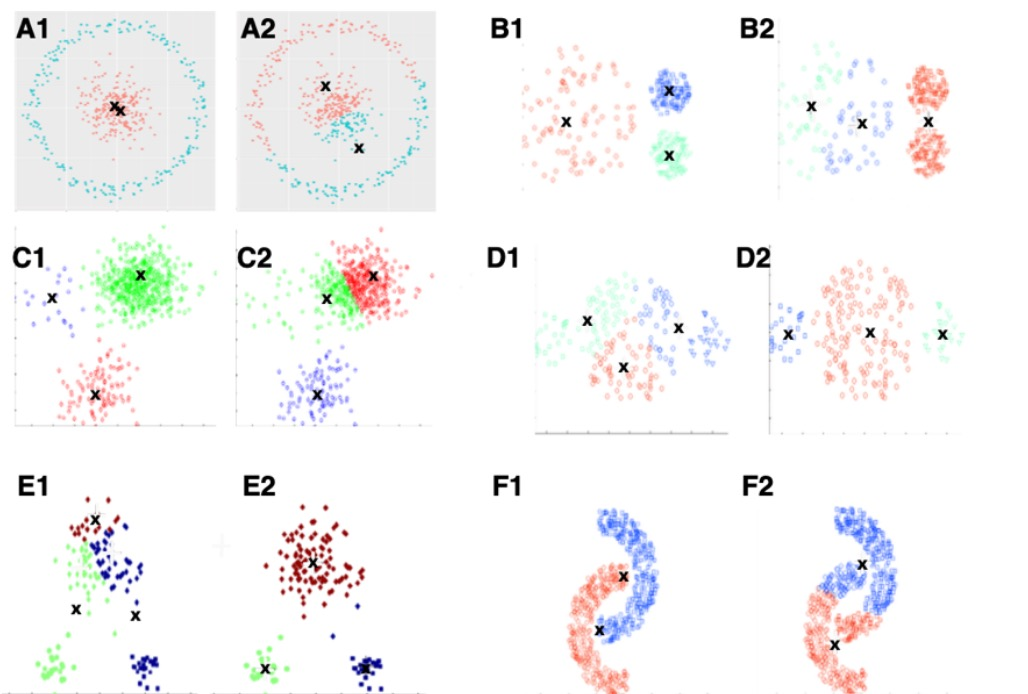
\includegraphics[width=0.6\textwidth]{images/title/聚类结果.jpg}
		\caption{聚类结果}
		\label{fig:聚类结果}
	\end{figure}

	\solution
	\begin{itemize}
		\item 对于$A$, 其中$A_2$很可能是$K$均值的聚类结果, 因为$A_1$的是非球形簇而$A_2$是球形簇. 由于图中的簇形状较为任意, 所以应该采用DBSCAN聚类算法;
		\item 对于$B$, 其中$B_2$最可能是$K$均值的聚类结果, 因为$K$均值聚类会受到不同密度的影响, 故应该采用DBSCAN聚类算法;
		\item 对于$C$, 其中$C_2$最可能是$K$均值的聚类结果, 因为$K$均值聚类会受到不同密度的影响, 故应该采用DBSCAN聚类算法;
		\item 对于$D$, 其中$D_1$最可能是$K$均值的聚类结果, 因为$K$均值聚类会受到不同尺寸(即先验概率)的影响, 而且簇都是球形簇, 故应该采用GMM-EM聚类算法;
		\item 对于$E$, 其中$E_1$最可能是$K$均值的聚类结果, 因为$K$均值聚类会受到不同尺寸(即先验概率)的影响, 而且簇都是球形簇, 故应该采用GMM-EM聚类算法;
		\item 对于$F$, 其中$F_2$很可能是$K$均值的聚类结果(这是由于$K$均值聚类只能针对球形/凸簇), 因为图中的簇形状较为任意, 所以应该采用DBSCAN聚类算法.
	\end{itemize}
\end{homeworkProblem}

\pagebreak






\begin{homeworkProblem}
	对如下图\ref{fig:聚类数据集}所示的数据集, 采用$K$均值聚类. 设$K=3$, 3个聚类中心分别为
	$$
	\mu _1=\left( 6.2,3.2 \right) ^{\text{T}}\left( {\color{red} \text{红色}} \right) ,\quad \mu _2=\left( 6.6,3.7 \right) ^{\text{T}}\left( {\color{green} \text{绿色}} \right) ,\quad \mu _3=\left( 6.5,3.0 \right) ^{\text{T}}\left( {\color{blue} \text{蓝色}} \right) 
	$$
	请给出一次迭代后属于第一簇的样本以及更新后的簇中心(保留两位小数).
	\begin{figure}[H]  % 这里记得用[H]
		\centering
		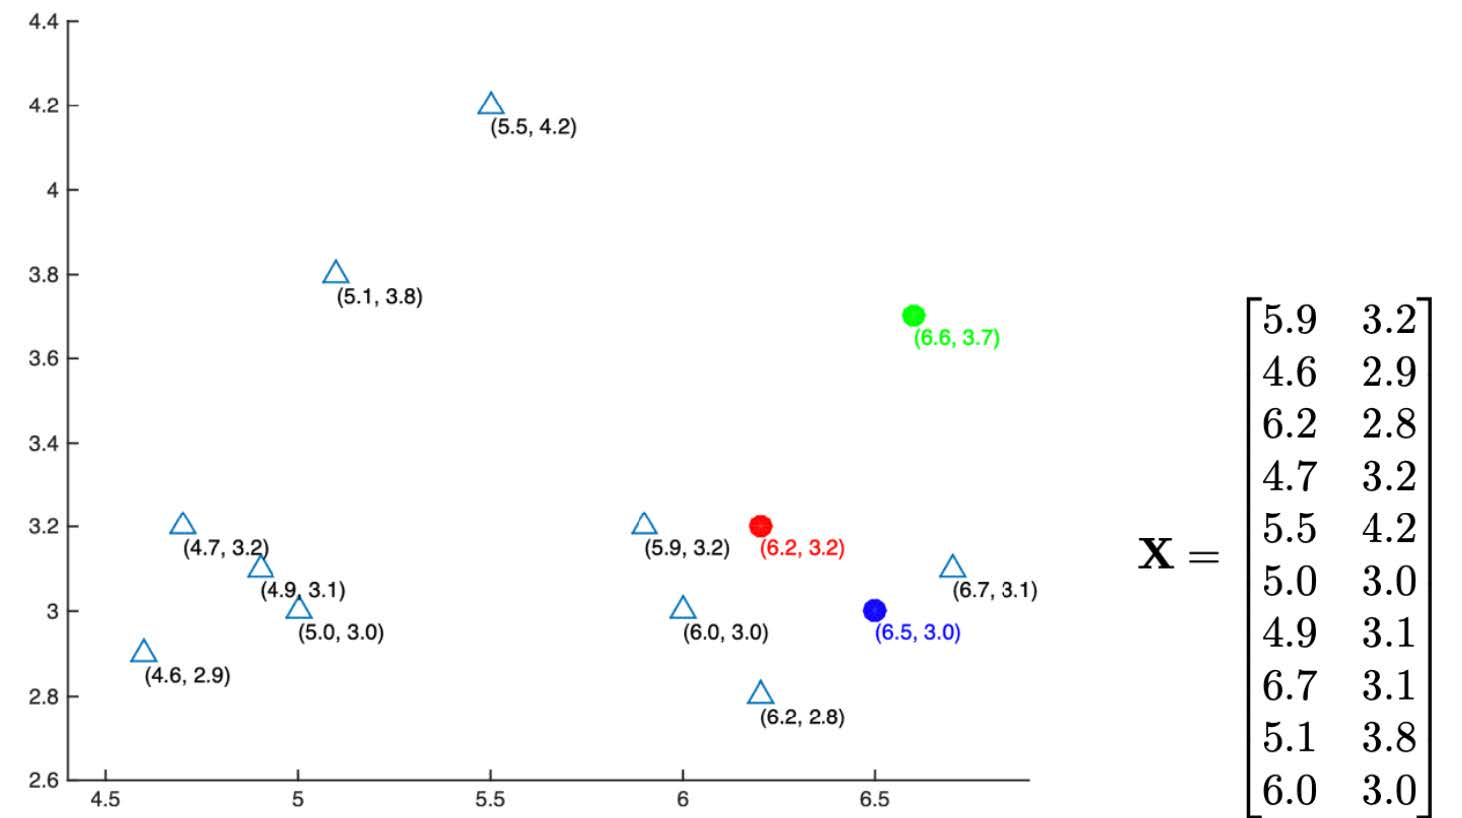
\includegraphics[width=0.7\textwidth]{images/title/数据集.jpg}
		\caption{聚类数据集}
		\label{fig:聚类数据集}
	\end{figure}
	
	\solution $K$-means聚类算法的流程见如下伪代码\ref{alg:K-means}:
	\begin{algorithm}[H]
		\begin{algorithmic}[1]
		\Require{给定$N$个样本点$\mathcal{D} =\left\{ \boldsymbol{x}_1,\boldsymbol{x}_2,\cdots ,\boldsymbol{x}_N \right\}	$}
		\Ensure{$K$个簇}
		\State 初始化选择$K$个种子数据点(seeds)作为$K$个簇的中心;
		\While{当前簇中心仍在更新}
			\For{each $\boldsymbol{x}_i\in \mathcal{D}$}
				\State 计算$\boldsymbol{x}_i$与每一个簇中心的距离;
				\State 将$\boldsymbol{x}_i$指配到距离最近的簇中心;
			\EndFor
			\State 用当前簇内点重新计算$K$个簇中心位置;
		\EndWhile
		\State \textbf{end \{K-means\}}
		\end{algorithmic}
		\caption{\textbf{K-means}算法}
		\label{alg:K-means}
	\end{algorithm}
	我们可以写出对应的C++代码来自动求出结果, 对应结果如下:

	第一轮迭代后属于第一簇的样本有$$\boldsymbol{x}_1,\boldsymbol{x}_2,\boldsymbol{x}_4,\boldsymbol{x}_6,\boldsymbol{x}_7,\boldsymbol{x}_9,\boldsymbol{x}_{10}$$
	且更新后的簇中心坐标为
	$$
	\mu _1=\left( 5.17,3.17 \right) ^{\text{T}},\quad \mu _2=\left( 5.50,4.20 \right) ^{\text{T}},\quad \mu _3=\left( 6.45,2.95 \right) ^{\text{T}}
	$$
	具体的C++代码如下:
\begin{tcblisting}{listing engine=minted,boxrule=0.1mm,
colback=blue!5!white,colframe=blue!75!black,
listing only,left=5mm,enhanced,sharp corners=all,
overlay={\begin{tcbclipinterior}\fill[red!20!blue!20!white] (frame.south west)
rectangle ([xshift=5mm]frame.north west);\end{tcbclipinterior}},
minted language=c++,
minted style=tango,
minted options={fontsize=\small,breaklines,autogobble,linenos,numbersep=3mm}}
#include <bits/stdc++.h> //万能头, 刷题可以用, 大型项目不要用
using namespace std;
double Distan(vector<double> &X, vector<double> &Y) {
    int L = X.size();
    double sum = 0;
    for(int i = 0; i < L; i++) {
        sum += pow(X[i] - Y[i], 2);
    }
    return sqrt(sum);
}

vector<int> ClusterLabel(vector<vector<double>> &Data, vector<vector<double>> &center) {
    vector<int> res;
    for(int i = 0; i < Data.size(); i++) {
        double dis1 = Distan(Data[i], center[0]);
        double dis2 = Distan(Data[i], center[1]);
        double dis3 = Distan(Data[i], center[2]);
        double dis = min(dis1, min(dis2, dis3));
        if(dis == dis1) res.push_back(1);
        else if(dis == dis2) res.push_back(2);
        else res.push_back(3);
    }
    return res;
}

vector<vector<double>> ClusterCenter(vector<vector<double>> &Data, vector<int> &label) {
    double cen1_x = 0, cen1_y = 0, cen2_x = 0, cen2_y = 0, cen3_x = 0, cen3_y = 0;
    int cnt1 = 0, cnt2 = 0, cnt3 = 0;
    for(int i = 0; i < Data.size(); i++) {
        if(label[i] == 1) {
            cen1_x += Data[i][0];
            cen1_y += Data[i][1];
            cnt1++;
        }
        else if(label[i] == 2){
            cen2_x += Data[i][0];
            cen2_y += Data[i][1];
            cnt2++; 
        }
        else {
            cen3_x += Data[i][0];
            cen3_y += Data[i][1];
            cnt3++;
        }
    }
    return {
        {cen1_x / cnt1, cen1_y / cnt1}, 
        {cen2_x / cnt2, cen2_y / cnt2}, 
        {cen3_x / cnt3, cen3_y / cnt3}
    };
}
\end{tcblisting}

主函数执行如下:
\begin{tcblisting}{listing engine=minted,boxrule=0.1mm,
colback=blue!5!white,colframe=blue!75!black,
listing only,left=5mm,enhanced,sharp corners=all,
overlay={\begin{tcbclipinterior}\fill[red!20!blue!20!white] (frame.south west)
rectangle ([xshift=5mm]frame.north west);\end{tcbclipinterior}},
minted language=c++,
minted style=tango,
minted options={fontsize=\small,breaklines,autogobble,linenos,numbersep=3mm}}
int main() {
    vector<vector<double>> Data = {
        {5.9, 3.2}, {4.6, 2.9}, {6.2, 2.8}, {4.7, 3.2}, {5.5, 4.2},
        {5.0, 3.0}, {4.9, 3.1}, {6.7, 3.1}, {5.1, 3.8}, {6.0, 3.0}
    };
    vector<vector<double>> center = {
        {6.2, 3.2}, {6.6, 3.7}, {6.5, 3.0}
    };
    vector<int> label = ClusterLabel(Data, center);
    for(int i = 0; i < Data.size(); i++) {
        cout << "第" << i + 1 << "个样本(" << Data[i][0] << "," 
        << Data[i][1] << ")属于第" << label[i] << "个簇" << endl; 
    }
    vector<vector<double>> NewCenter = ClusterCenter(Data, label);
    for(int i = 0; i < 3; i++) {
        cout << "第" << i + 1 << "个簇中心坐标为("
        << setprecision(3) << NewCenter[i][0] <<"," << 
        setprecision(3) << NewCenter[i][1] << ")" << endl;
    }
}
\end{tcblisting}


	具体的C++代码输出如下:
\begin{tcblisting}{listing engine=minted,boxrule=0.1mm,
colback=blue!5!white,colframe=blue!75!black,
listing only,left=5mm,enhanced,sharp corners=all,
overlay={\begin{tcbclipinterior}\fill[red!20!blue!20!white] (frame.south west)
rectangle ([xshift=5mm]frame.north west);\end{tcbclipinterior}},
minted language=c++,
minted style=tango,
minted options={fontsize=\small,breaklines,autogobble,linenos,numbersep=3mm}}
开始运行...
第1个样本(5.9,3.2)属于第1个簇
第2个样本(4.6,2.9)属于第1个簇
第3个样本(6.2,2.8)属于第3个簇
第4个样本(4.7,3.2)属于第1个簇
第5个样本(5.5,4.2)属于第2个簇
第6个样本(5,3)属于第1个簇
第7个样本(4.9,3.1)属于第1个簇
第8个样本(6.7,3.1)属于第3个簇
第9个样本(5.1,3.8)属于第1个簇
第10个样本(6,3)属于第1个簇
第1个簇中心坐标为(5.17,3.17)
第2个簇中心坐标为(5.5,4.2)
第3个簇中心坐标为(6.45,2.95)
运行结束.
\end{tcblisting}
\end{homeworkProblem}











\pagebreak

\begin{homeworkProblem}
	\textbf{简答题:}
	\begin{itemize}
		\item \textbf{问题1: K-means聚类算法暗含了对簇的什么假设?}
		
		\textbf{解答:} K-means聚类算法暗含了各个簇种的数据具有一样的先验概率并且呈现球形分布.
		\item \textbf{问题2: K-means迭代一定会收敛么?}
		
		\textbf{解答:} 一定会, 这是因为损失函数是单调递减的, 所以使用坐标轴下降法是可以使得损失函数收敛(但不一定收敛到全局极小值)且聚类结果也会收敛.
		\item \textbf{问题3: K-means算法的初始化参数(中心)如何选取?}
		
		\textbf{解答:} 采用启发式做法, 即随机确定第一个类的中心, 其他类中心的位置尽量远离已有类中心. 具体做法是在Scikit-Learn里K-means的参数init中设置“k-means++”(默认值)来使得初始化的质心彼此远离.
		\item \textbf{问题4: K-means算法的超参数$K$如何选取?}
		
		\textbf{解答:} 可以用手肘法, 观察出损失函数的拐点(急速下降和平稳的交界处), 对应的横坐标值即可作为$K$值. 此外还可以用间隔统计法来获取合适的$K$值, 具体代码可见\href{https://github.com/milesgranger/gap_statistic}{\textbf{Python implementation of the Gap Statistic}}.
		\item \textbf{问题5: K均值算法有何局限性? 可以用什么方法改进?}
		
		\textbf{解答:} K-means的局限性在于它假定了簇为球形并且各个簇的先验概率相等. 当各个簇是具有不同尺寸、密度的非球形簇时, 聚类效果不理想, 并且该算法易受到离群点的影响. 为此, 可以用簇的中位点来替代作为中心的均值点, 以免算法受到脏数据的干扰. 而针对先验概率相等的假设问题, 我们可以使用高斯混合模型来解决.
		\item \textbf{问题6: 基于GMM的EM聚类算法为何要引入隐变量$z$?}
		
		\textbf{解答:} 不引入隐变量$z$的话, 对数似然函数求导困难从而使得函数优化困难. 因此引入隐变量$z$, 从而给出隶属度$\gamma(z_{ik})$以求得对数似然的极大估计$\boldsymbol{\mu}_k,\pi_k,\boldsymbol{\Sigma}_k$. 于是可以引出解的迭代方案(即EM算法在GMM下的实例).
		\item \textbf{问题7: K-means和EM算法有什么共通之处?}
		
		\textbf{解答:} GMM的E步时软划分版本的K-means, 当所有$\pi_k$相等(即$1/k$)且$\boldsymbol{\Sigma}_k=\boldsymbol{O},r_{ik}\in \{0,1\}$时, 则GMM的EM算法退化为K-means算法.
		\item \textbf{问题8: 如何度量簇的相似性? 不同度量方法的优缺点?}
		
		\textbf{解答:} 簇的相似性可以用\textit{Minkowski}距离、余弦相似度、\textit{Pearson}相关系数以及\textit{Jaccard}相似系数来度量. 其中\textit{Minkowski}距离的优点在于对样本特征的旋转和平移比较鲁棒, 但缺点在于对数据尺度比较敏感. 余弦相似度的优势在于文本分析, 缺点是没有考虑向量模长的大小, 而只考虑它们的方向. 其中数据中心化后的\textit{Pearson}相关系数就是余弦相似度, 优缺点是一致的. \textit{Jaccard}相似系数(即交比并)的优势在于处理图像分割问题(如实例和语义分割), 缺点在于它容易受到数据规模的影响.
		\item \textbf{问题9: 层次聚类的限制有哪些?}
		
		\textbf{解答:} 簇的合并/拆分过程不可逆、没有对应优化一个全局目标函数、对离群点和噪声不鲁棒.
		\item \textbf{问题10: 请简述PCA流程.}
		
		\textbf{解答:} PCA流程如算法\ref{alg:PCA}中所示:
		\begin{algorithm}[H]
			\begin{algorithmic}[1]
			\Require{训练数据集$\boldsymbol{X}=\left\{ \boldsymbol{x}_1,\boldsymbol{x}_2,\cdots ,\boldsymbol{x}_N \right\}$, 低维空间的维度$D'$}
			\Ensure{$\boldsymbol{W}=\left( \boldsymbol{w}_1,\boldsymbol{w}_2,\cdots ,\boldsymbol{w}_{D'} \right)$}
			\State 对样本中心化: $\displaystyle \boldsymbol{x}_i\gets \boldsymbol{x}_i-\frac{1}{N}\sum_{j=1}^N{\boldsymbol{x}_j},i=1,\cdots,N$;
			\State 再计算协方差矩阵$\boldsymbol{X}\boldsymbol{X}^{\text{T}}$;
			\State 对$\boldsymbol{X}\boldsymbol{X}^{\text{T}}$作特征分解: $\boldsymbol{XX}^{\text{T}}=\boldsymbol{W}\boldsymbol{\Sigma }\boldsymbol{W}^{-1}$;
			\State $D'$最大特征值对应的特征向量: $\boldsymbol{w}_1,\boldsymbol{w}_2,\cdots ,\boldsymbol{w}_{D'}$;
			\State \textbf{end \{PCA\}}
			\end{algorithmic}
			\caption{\textbf{PCA}算法}
			\label{alg:PCA}
		\end{algorithm}
		改进后的PCA流程如算法\ref{alg:PCA2}中所示:
		\begin{algorithm}[H]
			\begin{algorithmic}[1]
			\Require{训练数据集$\boldsymbol{X}=\left\{ \boldsymbol{x}_1,\boldsymbol{x}_2,\cdots ,\boldsymbol{x}_N \right\}$, 低维空间的维度$D'$}
			\Ensure{$\boldsymbol{U}=\left( \boldsymbol{u}_1,\boldsymbol{u}_2,\cdots ,\boldsymbol{u}_{D'} \right)$}
			\State 对样本中心化: $\displaystyle \boldsymbol{x}_i\gets \boldsymbol{x}_i-\frac{1}{N}\sum_{j=1}^N{\boldsymbol{x}_j},i=1,\cdots,N$;
			\State 对$\boldsymbol{X}$作奇异值分解: $\boldsymbol{X}=\boldsymbol{U}_{D\times D}\boldsymbol{\Sigma} _{D\times N}\boldsymbol{V}_{N\times N}^{\text{T}}$;
			\State $D'$个奇异值对应的左奇异向量: $\boldsymbol{u}_1,\boldsymbol{u}_2,\cdots ,\boldsymbol{u}_{D'}$;
			\State \textbf{end \{Improved PCA\}}
			\end{algorithmic}
			\caption{改进\textbf{PCA}算法}
			\label{alg:PCA2}
		\end{algorithm}
		KPCA流程如算法\ref{alg:KPCA}中所示:
		\begin{algorithm}[H]
			\begin{algorithmic}[1]
			\Require{训练数据集$\boldsymbol{X}=\left\{ \boldsymbol{x}_1,\boldsymbol{x}_2,\cdots ,\boldsymbol{x}_N \right\}$, 低维空间的维度$D'$, 核函数$k(\cdot,\cdot)$}
			\Ensure{$\boldsymbol{z}^{(i)}=\left( \boldsymbol{z}_1^{(i)},\boldsymbol{z}_2^{(i)},\cdots ,\boldsymbol{z}_{D'}^{(i)} \right)$,$i=1,\cdots,N$}
			\State 计算核矩阵$\boldsymbol{K}$: $k_{ij}=k(\boldsymbol{x}_i,\boldsymbol{x}_j)$并对$\boldsymbol{K}$中心化得到$\overline{\boldsymbol{K}}$;
			\State 对$\overline{\boldsymbol{K}}$作特征分解: $\overline{\boldsymbol{K}}=\boldsymbol{\mathcal{A}} \boldsymbol{\Sigma }\boldsymbol{\mathcal{A}} ^{-1}$;
			\State 选择$D'$个最大特征值对应的特征向量: $\boldsymbol{\alpha}_1,\cdots ,\boldsymbol{\alpha}_{D'}$; \Comment{$\boldsymbol{\alpha}\in \mathbb{R}^{N\times 1}$, 通常对$\boldsymbol{\alpha}$进行归一化, 模长为1}
			\State 对于新样本$\boldsymbol{x}$, 可得到其低维表示($D'$维)$\boldsymbol{z}$为: \Comment{对所有样本求和开销大}
			$$
			\boldsymbol{z}=\left( \begin{array}{c}
				\displaystyle \sum_{i=1}^N{\alpha _{1i}k\left( \boldsymbol{x}_i,\boldsymbol{x} \right)}\\
				\displaystyle \sum_{i=1}^N{\alpha _{2i}k\left( \boldsymbol{x}_i,\boldsymbol{x} \right)}\\
				\vdots\\
				\displaystyle \sum_{i=1}^N{\alpha _{D'i}k\left( \boldsymbol{x}_i,\boldsymbol{x} \right)}\\
			\end{array} \right)
			$$
			\State \textbf{end \{KPCA\}}
			\end{algorithmic}
			\caption{\textbf{KPCA}算法}
			\label{alg:KPCA}
		\end{algorithm}
	\end{itemize}
\end{homeworkProblem}


% 引用文献
%\bibliographystyle{unsrt}  % unsrt:根据引用顺序编号
%\bibliography{refs}


\end{document}
